% Intended LaTeX compiler: pdflatex
\documentclass[10pt,a4paper,UTF8]{article}
\usepackage{zclorg}
\usepackage{tikztheorem}
\author{emacsun}
\date{}
\title{Thinking in Java chapter8 类重用}
\hypersetup{
 pdfauthor={emacsun},
 pdftitle={Thinking in Java chapter8 类重用},
 pdfkeywords={},
 pdfsubject={},
 pdfcreator={Emacs 25.0.50.1 (Org mode 9.0.6)},
 pdflang={English}}
\begin{document}

\maketitle
\tableofcontents
\titlepic{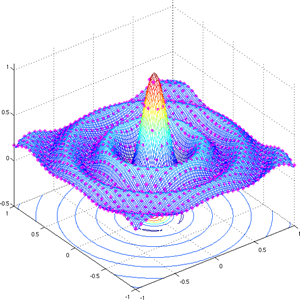
\includegraphics[scale=0.25]{../../img/sinc.PNG}}

\section{简介}
\label{sec:orgedcfd59}


Java的一个重要的特性就是可以方便的实现类重用。重用代码的概念在编程语言里早有体现:把常用的相对独立的功能以函数的形式保存,以备以后调用而不是重新编写。在Java语言中,重用代码的概念通过类重用得到了进一步的延伸。

今天我们学习两种代码重用的技巧: \texttt{composition} 和 \texttt{inheritance} 。我们简单的把 \texttt{composition} 翻译成为 组合,把 \texttt{inheritance} 翻译为继承。大多时候我都倾向于保持使用 \texttt{composition} 和 \texttt{inheritance} ,这样一来虽然避免技术词汇翻译带来的不同意,但是却带来了语言的不中不洋。考虑到我们以技术讨论为主,我觉得保持技术文献的不中不洋没有什么不妥。

\section{\texttt{composition}}
\label{sec:org4a9b159}


我们之前就接触过 \texttt{composition} 这种代码重用方式。简而言之, \texttt{composition} 就是在一个类中生成另一个类的对象。

我们用一个例子来说明这个问题:
\lstset{language=C,label= ,caption= ,captionpos=b,firstnumber=1,numbers=left}
\begin{lstlisting}
//: reusing/SprinklerSystem.java
// Composition for code reuse.

class WaterSource {
  private String s;
  WaterSource() {
    System.out.println("WaterSource()");
    s = "Constructed";
  }
  public String toString() { return s; }
}

public class SprinklerSystem {
  private String valve1, valve2, valve3, valve4;
  private WaterSource source = new WaterSource();
  private int i;
  private float f;
  public String toString() {
    return
      "valve1 = " + valve1 + " " +
      "valve2 = " + valve2 + " " +
      "valve3 = " + valve3 + " " +
      "valve4 = " + valve4 + "\n" +
      "i = " + i + " " + "f = " + f + " " +
      "source = " + source;
  }
  public static void main(String[] args) {
    SprinklerSystem sprinklers = new SprinklerSystem();
    System.out.println(sprinklers);
  }
} /* Output:
\end{lstlisting}
在上面的例子中类 \texttt{SprinklerSystem} 具有几个私有变量,除了 \texttt{privimitive} 类型外还有一个 \texttt{WaterSource} 类型的类索引。这个类索引指向另一个类 \texttt{WaterSource} 。这就是 \texttt{composition} 。

在上面的例子中,我们还可以挖掘更多的东西。首先 \texttt{SprinklerSystem} 和 \texttt{WaterSource} 都定义了一个方法 \texttt{toString} 。当编译器需要一个 \texttt{String} 输入,但是给定的输入确实一个 object时,这个方法就会被调用。比如,在上面的例子中, \texttt{SprinklerSystem} 类中有一语句:
\lstset{language=java,label= ,caption= ,captionpos=b,numbers=none}
\begin{lstlisting}
"source = " + source;
\end{lstlisting}
编译器发现,你想把一个 \texttt{WaterSource} 对象与一个 \texttt{String} 相加。但是,我们知道只有 \texttt{String} 类型的才能相加。这个时候编译器就会得到一个消息:“调用 \texttt{toString} 把 \texttt{source} 变成 \texttt{String} ”。然后把 \texttt{toString} 的输出和  \texttt{"source = "} 相加。

任何时候,如果你想要实现这种字符串和对象的相加,都需要在类定义中定义方法 \texttt{toString} 。

上面一段代码的输出是:
\begin{verbatim}
WaterSource()
valve1 = null valve2 = null valve3 = null valve4 = null
i = 0 f = 0.0 source = Constructed
\end{verbatim}
我们看到字符串初始化为 \texttt{null} ,浮点数和整数初始化为 0.
\section{\texttt{inheritance}}
\label{sec:org4716ce1}


\texttt{inheritance} 是面向对象语言重要组成部分。 实际上在Java中,你无时无刻不在使用继承。即使不是显示的实用,你也在隐式的实用。Java的所有对象都之间或者间接的继承于一个类 \texttt{Object} 。 在Java中使用 \texttt{extends} 来扩展原来的类(我们称之为基类)。

接下来我们通过一个例子来了解 \texttt{inheritance} 的语法。

\lstset{language=C,label= ,caption= ,captionpos=b,firstnumber=1,numbers=left}
\begin{lstlisting}
//: reusing/Detergent.java
// Inheritance syntax & properties.
package reusing;
import static net.mindview.util.Print.*;

class Cleanser {
    private String s = "Cleanser comes first";
    private String t = " Cleanser comes second";
    private String u = " Cleanser comes third";
    public void append(String a) { s += t;s+=a; }
    public void dilute() { append(" dilute()"); }
    public void apply() { append(" apply()"); }
    public void scrub() { append(" scrub()"); }
    public String toString() { return s; }
    public static void main(String[] args) {
        Cleanser x = new Cleanser();
        x.dilute(); x.apply(); x.scrub();
        print(x);
    }
}

public class Detergent extends Cleanser {
    // Change a method:
    public void scrub() {
        append(" Detergent.scrub()");
        super.scrub(); // Call base-class version
    }
    // Add methods to the interface:
    public void foam() { append(" foam()"); }
    // Test the new class:
    public static void main(String[] args) {
        Detergent x = new Detergent();
        x.dilute();
        x.apply();
        x.scrub();
        x.foam();
        print(x);
        print("Testing base class:");
        Cleanser.main(args);
    }
} /* Output:
     Cleanser dilute() apply() Detergent.scrub() scrub() foam()
     Testing base class:
     Cleanser dilute() apply() scrub()
  *///:~
\end{lstlisting}
在这个例子中 \texttt{Cleanser} 是基类, \texttt{Detergent} 是对基类的扩展。注意关键词 \texttt{extends} 。

上面的例子中有几点需要我们特别注意。首先在 \texttt{Cleanser append()} 中 \texttt{String} 类型通过操作符 \texttt{+=} 来实现连接,这对操作符 \texttt{+=} 的重载。

第二,在 \texttt{Cleanser} 和 \texttt{Detergent} 中都有 \texttt{main} 函数。这种在每个类中放一个 \texttt{main} 的做法有助于测试每一个类的功能。如果在一个java程序中有很多的类,意味着可能有多个 \texttt{main} 函数。只有命令行调用的那个类能够执行。在上面的代码中,只有 \texttt{Detergent.main()} 会被调用。

第三,在 \texttt{Detergent.main()} 中显示的调用了 \texttt{Cleanser.main()} 。传给 \texttt{Cleanser.main()} 的参数,和传给 \texttt{Detergent.main()} 的参数是一样的。

在 \texttt{Cleanser} 中的所有方法都是 \texttt{public} 的。如果对这些函数不指定 \texttt{public} 或者 \texttt{private} 这样的约束,这些函数的默认访问方式是 \texttt{package access} .也就是说这些函数只允许 \texttt{package} 的成员访问,也就是说在这个 \texttt{package} 中,任何一个类都可以访问这些成员函数。 \texttt{Detergent} 类在访问 \texttt{Cleanser} 类的方法过程中,即使 \texttt{Cleanser} 类中的方法没有指定 \texttt{public} 也不要紧,因为可以通过 \texttt{package access} 访问。但是假设如果其他 \texttt{package} 中的类(继承自 \texttt{Detergent} )想要访问 \texttt{Detergent} 类中的方法,它只能访问 \texttt{Detergent} 中带有 \texttt{public} 标识的方法 。一个通用的规则是,把一个类中的数据私有化(打上 \texttt{private} 标签 ),把方法公有化(打上 \texttt{public} 标签)。

在 \texttt{Detergent} 类中,重新定义了 \texttt{scrub} 函数(),注意到在基类 \texttt{Cleanser} 中也定义了 \texttt{scrub} 。那么在 \texttt{Detergent} 访问的 \texttt{scrub} 函数是在 \texttt{Detergent} 类中定义的。如果此时我想访问基类中的 \texttt{scrub} 函数怎么办?有个关键词 \texttt{super} .就像在 \texttt{Detergent} 的 \texttt{scrub} 函数中那样 \texttt{super.scrub()} . 显然,通过使用 \texttt{inheritance} ,在继承类中,我们不仅可以使用基类中的方法,也可以重新定义相同名字的方法,并通过 \texttt{super} 来访问基类中定义的方法。
\end{document}
